\documentclass[10pt,dvipsnames]{beamer}
\usepackage{amsmath,amssymb,longtable,hhline}
\usepackage{mathrsfs}
\usepackage{xcolor}
\usepackage{hyperref}
\usepackage{multicol}
\usepackage{anyfontsize}
\usepackage{minted}

\usemintedstyle{tango}
\newcommand{\ltprgsize}{\fontsize{5}{5}\selectfont}
\setminted{fontsize=\ltprgsize,mathescape}

\definecolor{mygreen}{rgb}{0,0.6,0}
\definecolor{mygray}{rgb}{0.5,0.5,0.5}
\definecolor{mymauve}{rgb}{0.58,0,0.82}

\hypersetup{
    bookmarks=true,         % show bookmarks bar?
    unicode=true,           % non-Latin characters in Acrobat’s bookmarks
    pdftoolbar=false,        % show Acrobat’s toolbar?
    pdfmenubar=false,        % show Acrobat’s menu?
    pdffitwindow=false,     % window fit to page when opened
    pdfstartview={FitH},    % fits the width of the page to the window
    pdftitle={Компьютерная алгебра в задачах оптимизации},    % title
    pdfauthor={Evgeny Cherkashin, Seseg Badmatsyrenova},     % author
    pdfsubject={symbolic computations},   % subject of the document
    pdfnewwindow=true,      % links in new PDF window
    colorlinks=true,       % false: boxed links; true: colored links
    linkcolor=red,          % color of internal links (change box color with linkbordercolor)
    citecolor=green,        % color of links to bibliography
    filecolor=magenta,      % color of file links
    urlcolor=blue           % color of external links
}

\usepackage{pifont}

\usetheme{Warsaw}
\usecolortheme{crane}
%\useinnertheme{rectangles}
\setbeamertemplate{itemize item}{\scriptsize\hbox{\donotcoloroutermaths\ding{113}}}
\setbeamertemplate{itemize subitem}{\tiny\raise1.5pt\hbox{\donotcoloroutermaths$\blacktriangleright$}}
\setbeamertemplate{itemize subsubitem}{\tiny\raise1.5pt\hbox{\donotcoloroutermaths$\blacktriangleright$}}
\setbeamertemplate{enumerate item}{\insertenumlabel.}
\setbeamertemplate{enumerate subitem}{\insertenumlabel.\insertsubenumlabel}
\setbeamertemplate{enumerate subsubitem}{\insertenumlabel.\insertsubenumlabel.\insertsubsubenumlabel}
\setbeamertemplate{enumerate mini template}{\insertenumlabel}

\beamertemplatenavigationsymbolsempty

\usepackage{iftex,ifxetex}
\ifPDFTeX
  \usepackage[utf8]{inputenc}
  \usepackage[T1]{fontenc}
  \usepackage[russian]{babel}
  \usepackage{lmodern}
  \usefonttheme{serif}
\else
  \ifluatex
    \usepackage{unicode-math}
    \defaultfontfeatures{Ligatures=TeX,Numbers=OldStyle}
    \setmathfont{Latin Modern Math}
    \setsansfont{Linux Biolinum O}
    \setmonofont{Fira Mono}
    \usefonttheme{professionalfonts}
    % \setmathfont[
    %     Ligatures=TeX,
    %     Scale=MatchLowercase,
    %     math-style=upright,
    %     vargreek-shape=unicode
    %     ]{euler.otf}
  \fi
\fi

%\useoutertheme{split}
%\useinnertheme{rounded}
\setbeamertemplate{background canvas}[vertical shading][bottom=white!80!cyan!20,top=cyan!10]
%\setbeamertemplate{sidebar canvas left}[horizontal shading][left=white!40!black,right=black]

\graphicspath{{pics/}}


% --------------------------

\def\remph#1{\textcolor{Mahogany}{\bfseries #1}}

\begin{document}
\parindent=1em
\title{Two recommender systems: Technical decisions and session learned}
\author{
\def\and{, }
\remph{Evgeny~Cherkashin}\and
Viktoria Kopylova\and
Boris Shevchenko\and
Nikita Lukyanov}

\date{October, 16, 2020}
\institute{\textit{Matrosov Institute for System Dynamics and Control Theory of SB RAS}, Irkutsk, Russia,
  \href{mailto:eugeneai@icc.ru}{eugeneai@icc.ru}\\
  \textit{National research Irkutsk state technical university,} Irkutsk, Russia,
  \href{mailto:kopylovika@mail.ru}{kopylovika@mail.ru}}

\maketitle
% ----------------------------------------------------------------
\begin{frame}{Introduction}

  \emph{Recommender systems} (RS) are examples of \emph{decision support systems}. They are useful to support users with additional information and decision variants.  We consider two application domains:
  \begin{enumerate}
  \item real estate of a region, helping with selling real estate;
  \item choosing the specialty of a high school, analyzing entrant's social network profile.
\end{enumerate}
Both systems were developed within master degree at IIT\&DA, National research Irkutsk state technical university.



The first system deals with the problem of selling real estate: a flat, a room in a flat, a house.  Most of the objects on the market have similar characteristics in a class, the user interest is expressed with obvious characteristics like price, location, level, number of owners.  But the most interesting aspect of the problem is the special cases of realty like private family hotels, countryside houses, shops.  These are usually being sold for a long time, and the real estate firms utilize too many efforts for that.  The time spent to find new owner of the property is critical for the business: sellers have losses due paying the taxes for the estate being not utilized, buyers have no possibilities to invest available capital.   RS focusing user interest on the previously filtered subsets of the property, preliminary sorting by relevance, could speed up the sales.

Each school student sooner or later faces the problem of choice of a future specialty, university to enroll, and the set of courses to study.  Decisions made at this time significantly affect their future life, their job and career perspectives, families' life level.  Therefore, any help at this stage seems to be a necessary. In comparison to the real estate, where there is a whole industry supporting decision-making -- the services of realtors --, in this field the educational environment supports only an information provision service: students are given only career guidance, advertisement for the high school capabilities.  The student is on his/her own in the fundamental life decision.  Of course, parents and favorite mentors can supply the additional life experience examples helping to focus the analysis of the present conditions, but the actuality of their advices are generally of questions due to specifics of their experience, subjectivity, absence of the topical information of the present state of the labor market, scientific progress, \emph{etc}.
\end{frame}

\begin{frame}
  \frametitle{Ralated Works Summary}
\end{frame}

\begin{frame}
  \frametitle{Data Sources for Real Estate RS}
\end{frame}

\begin{frame}
  \frametitle{Data Sources for Entrants}
\end{frame}

\begin{frame}
  \frametitle{Used Technologies}

\end{frame}

\begin{frame}
  \frametitle{Classification of Realty Objects}

 \begin{columns}
    \begin{column}{0.8\linewidth}
\begin{table}[tb]
  \footnotesize
  \centering
  \begin{tabular}{|l|l|c|c|}
    \hline
    Attribute & Calculation technique & $v_k, \%$ & Formula \\
    \hline
\texttt{string Name} & not used & & \\
    \texttt{ILocation Location} & equality & 10 & $(\star)$
    \\
\texttt{string Address} & --''-- & 10 & \\
\texttt{float Price} & relative difference & 25 & $(\star\star)$\\
\texttt{float Area} & relative difference  & 35 & $(\star\star)$\\
\texttt{string ImageURL} & --''-- & & \\
\texttt{string URL} & --''-- & & \\
\texttt{int Rooms}  & relative difference  & 100 & $(\star\star)$\\
\texttt{int RoomsOffered} &  --''--   & 100 & $(\star\star)$\\
\texttt{int Floor}  &  --''--   & 30 & $(\star\star)$\\
\texttt{int FloorTotal}  &  --''--   & 10 & $(\star\star)$\\
\texttt{BuildingEnum \ldots}  & equality & 30 & $(\star)$\\
\texttt{IBuilding \ldots{}}  & --''-- & 30 &  $(\star)$\\
\texttt{PropertyEnum \ldots} & --''-- & 30 &  $(\star)$\\
\texttt{CategoryEnum \ldots} & --''-- & 100 &  $(\star)$\\
    \texttt{string GUID} & --''-- & & \\
    \hline
  \end{tabular}
  \end{table}
 \end{column}
\begin{column}{0.2\linewidth}\footnotesize
\[
  d_k(i,j) =
\]
\[
 =\left\{
                                                          \begin{array}{ll}
                                                            0, & \mbox{if\ \ } a_i=a_j,\\
                                                            1, & \mbox{if\ \ } a_i\neq a_j,
                                                          \end{array}
                                                        \right.
                                                      \]
                                                  \[
  (\star)
\]
\\[2em]
\[
  = \frac{|a_i^k-a_j^k|}{a_i^k+a_j^k},\] \[ a_i^k+a_j^k>0.
  \quad (\star\star)
\]
\end{column}
\end{columns}

\[
  d(i,j)=\frac{\sum\limits_{k=1}^m|v_k\cdot d_k(i,j)|}{\sum\limits_{k=1}^m v_k}, \qquad 0\leqslant d_{i,j}\leqslant 1,
\]
\noindent where $v_k$ is a weight of $k$-th attribute value, defined in the table.

\end{frame}

\begin{frame}
  \frametitle{Recommendations generation behavior}

   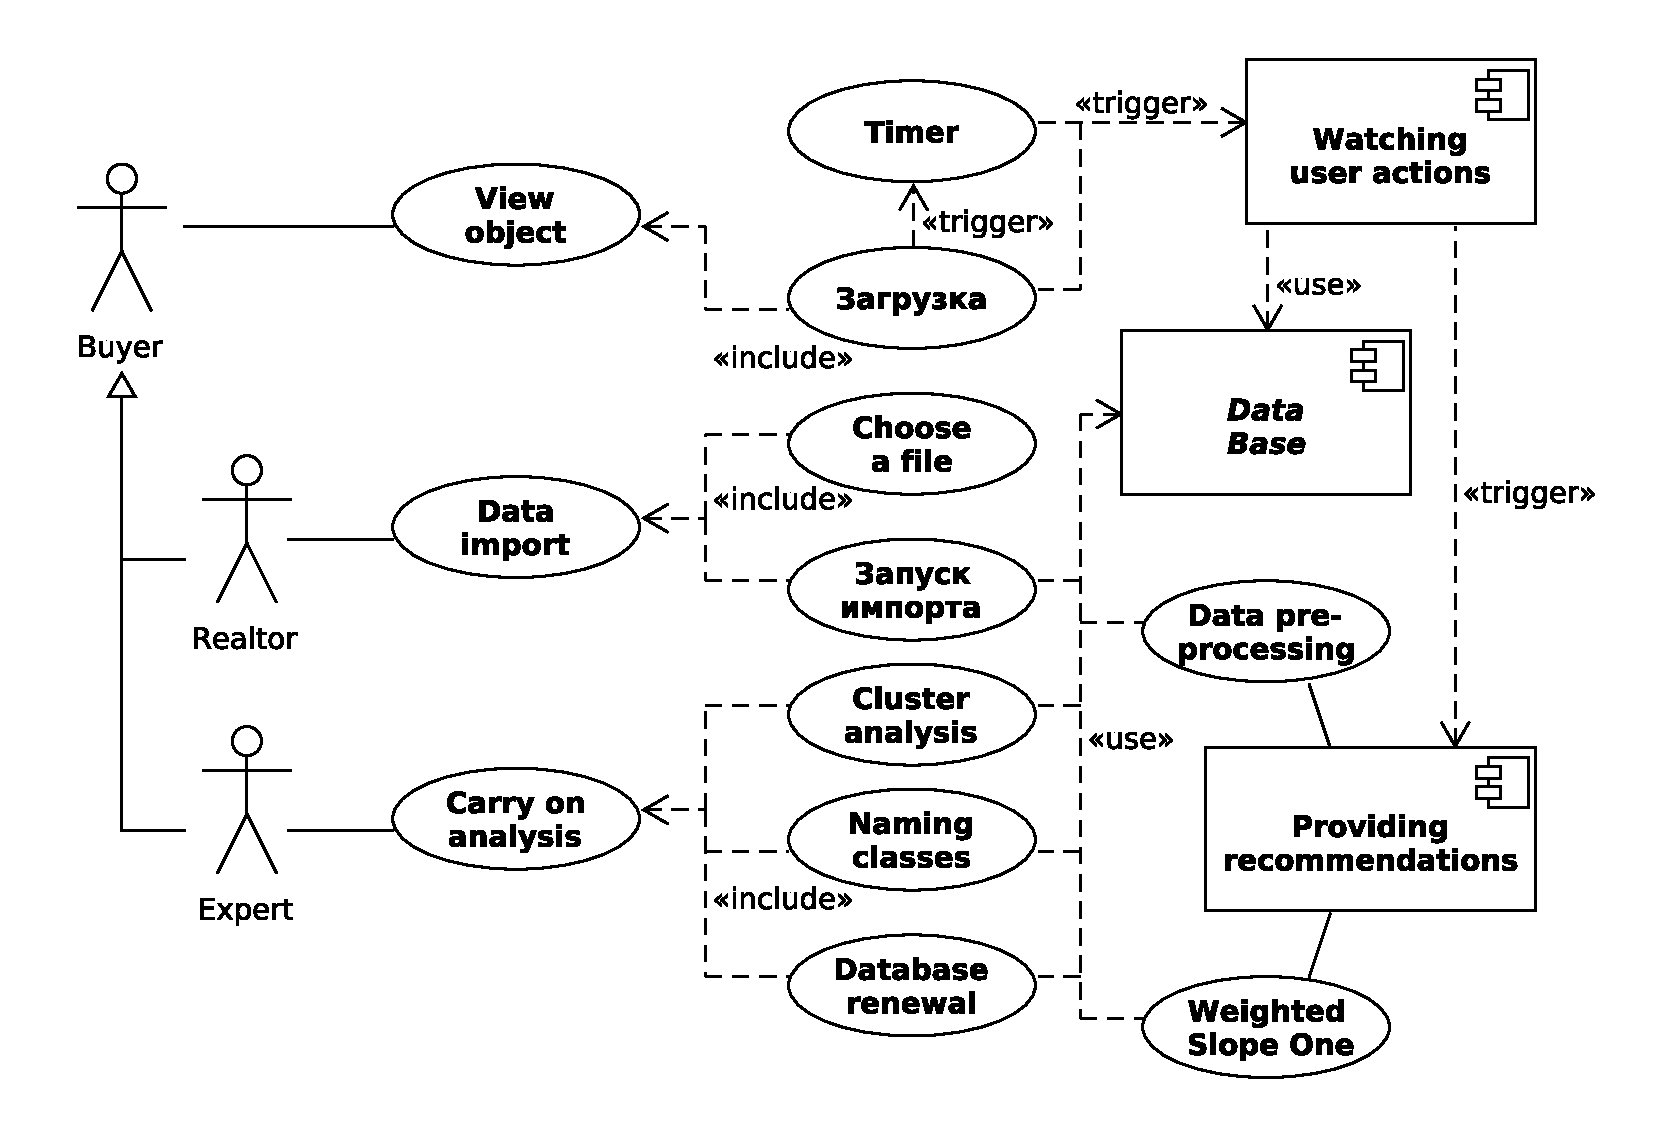
\includegraphics[width=1\linewidth]{use_case.eps}

\end{frame}

\begin{frame}
  \frametitle{Web Application}
  As the software platform of the RS is C\# we used ASP.NET based frameworks, such as \texttt{Nancy}, mapping an URL to a lambda function of one argument.

  HTTP template engine is based on SharpTAL, allowing implementation of MVC with a dictionary variable substitution.  It can be extended to support LOD cross-site integration.
\vfill\centering
  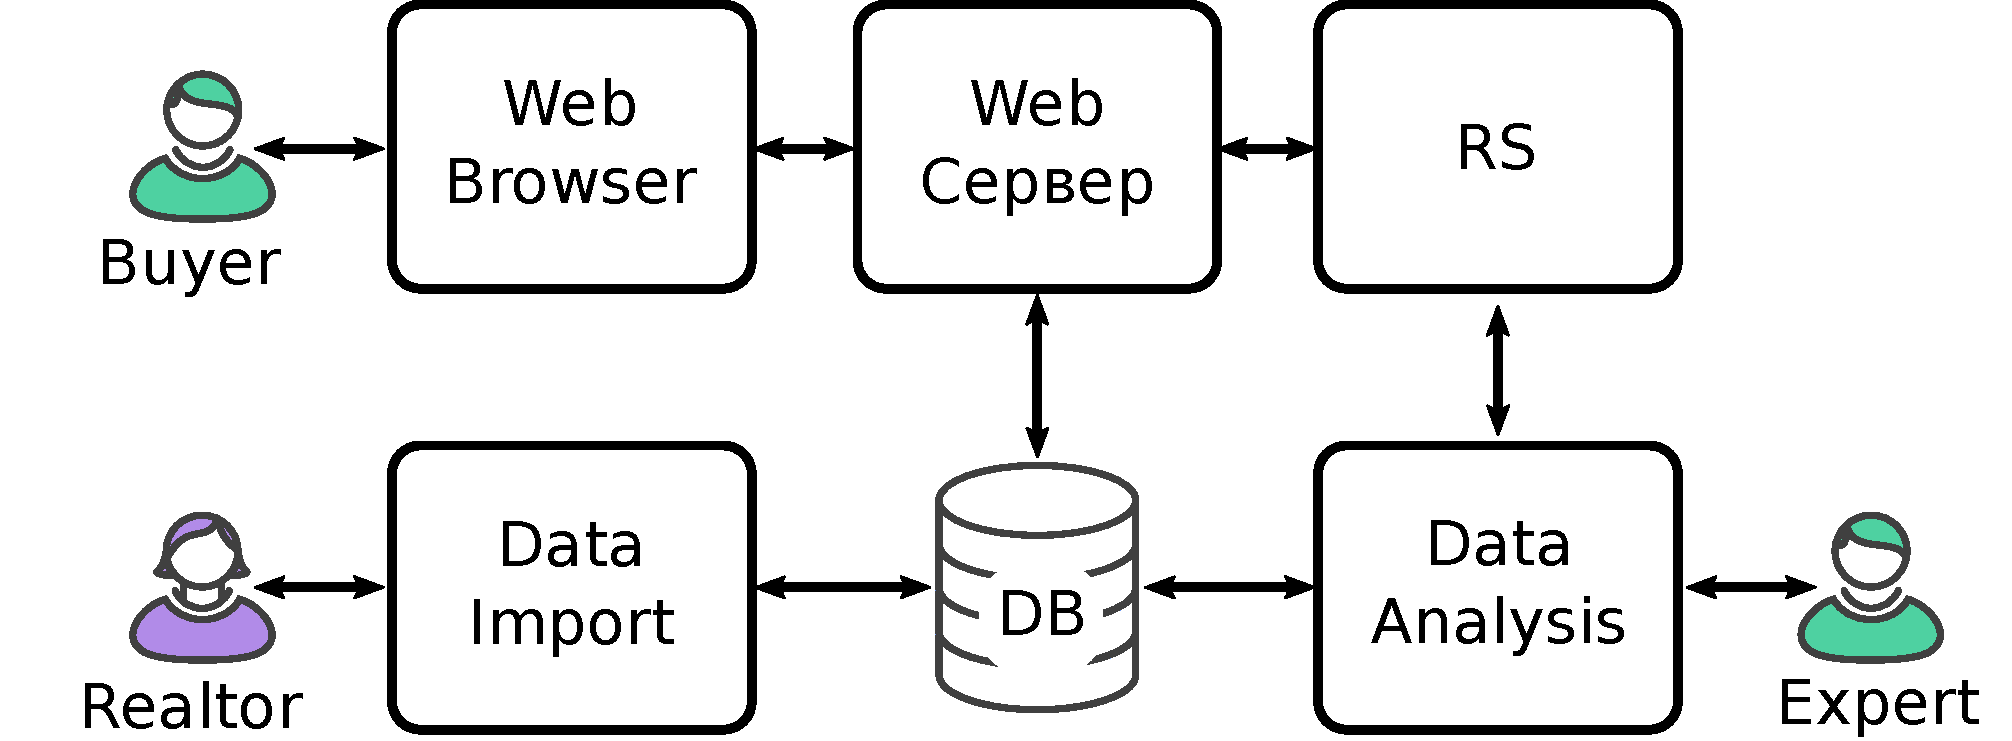
\includegraphics[width=1\linewidth]{architecture.pdf}

\end{frame}


\begin{frame}
  \frametitle{Persistent Object Structure}
   \centering
   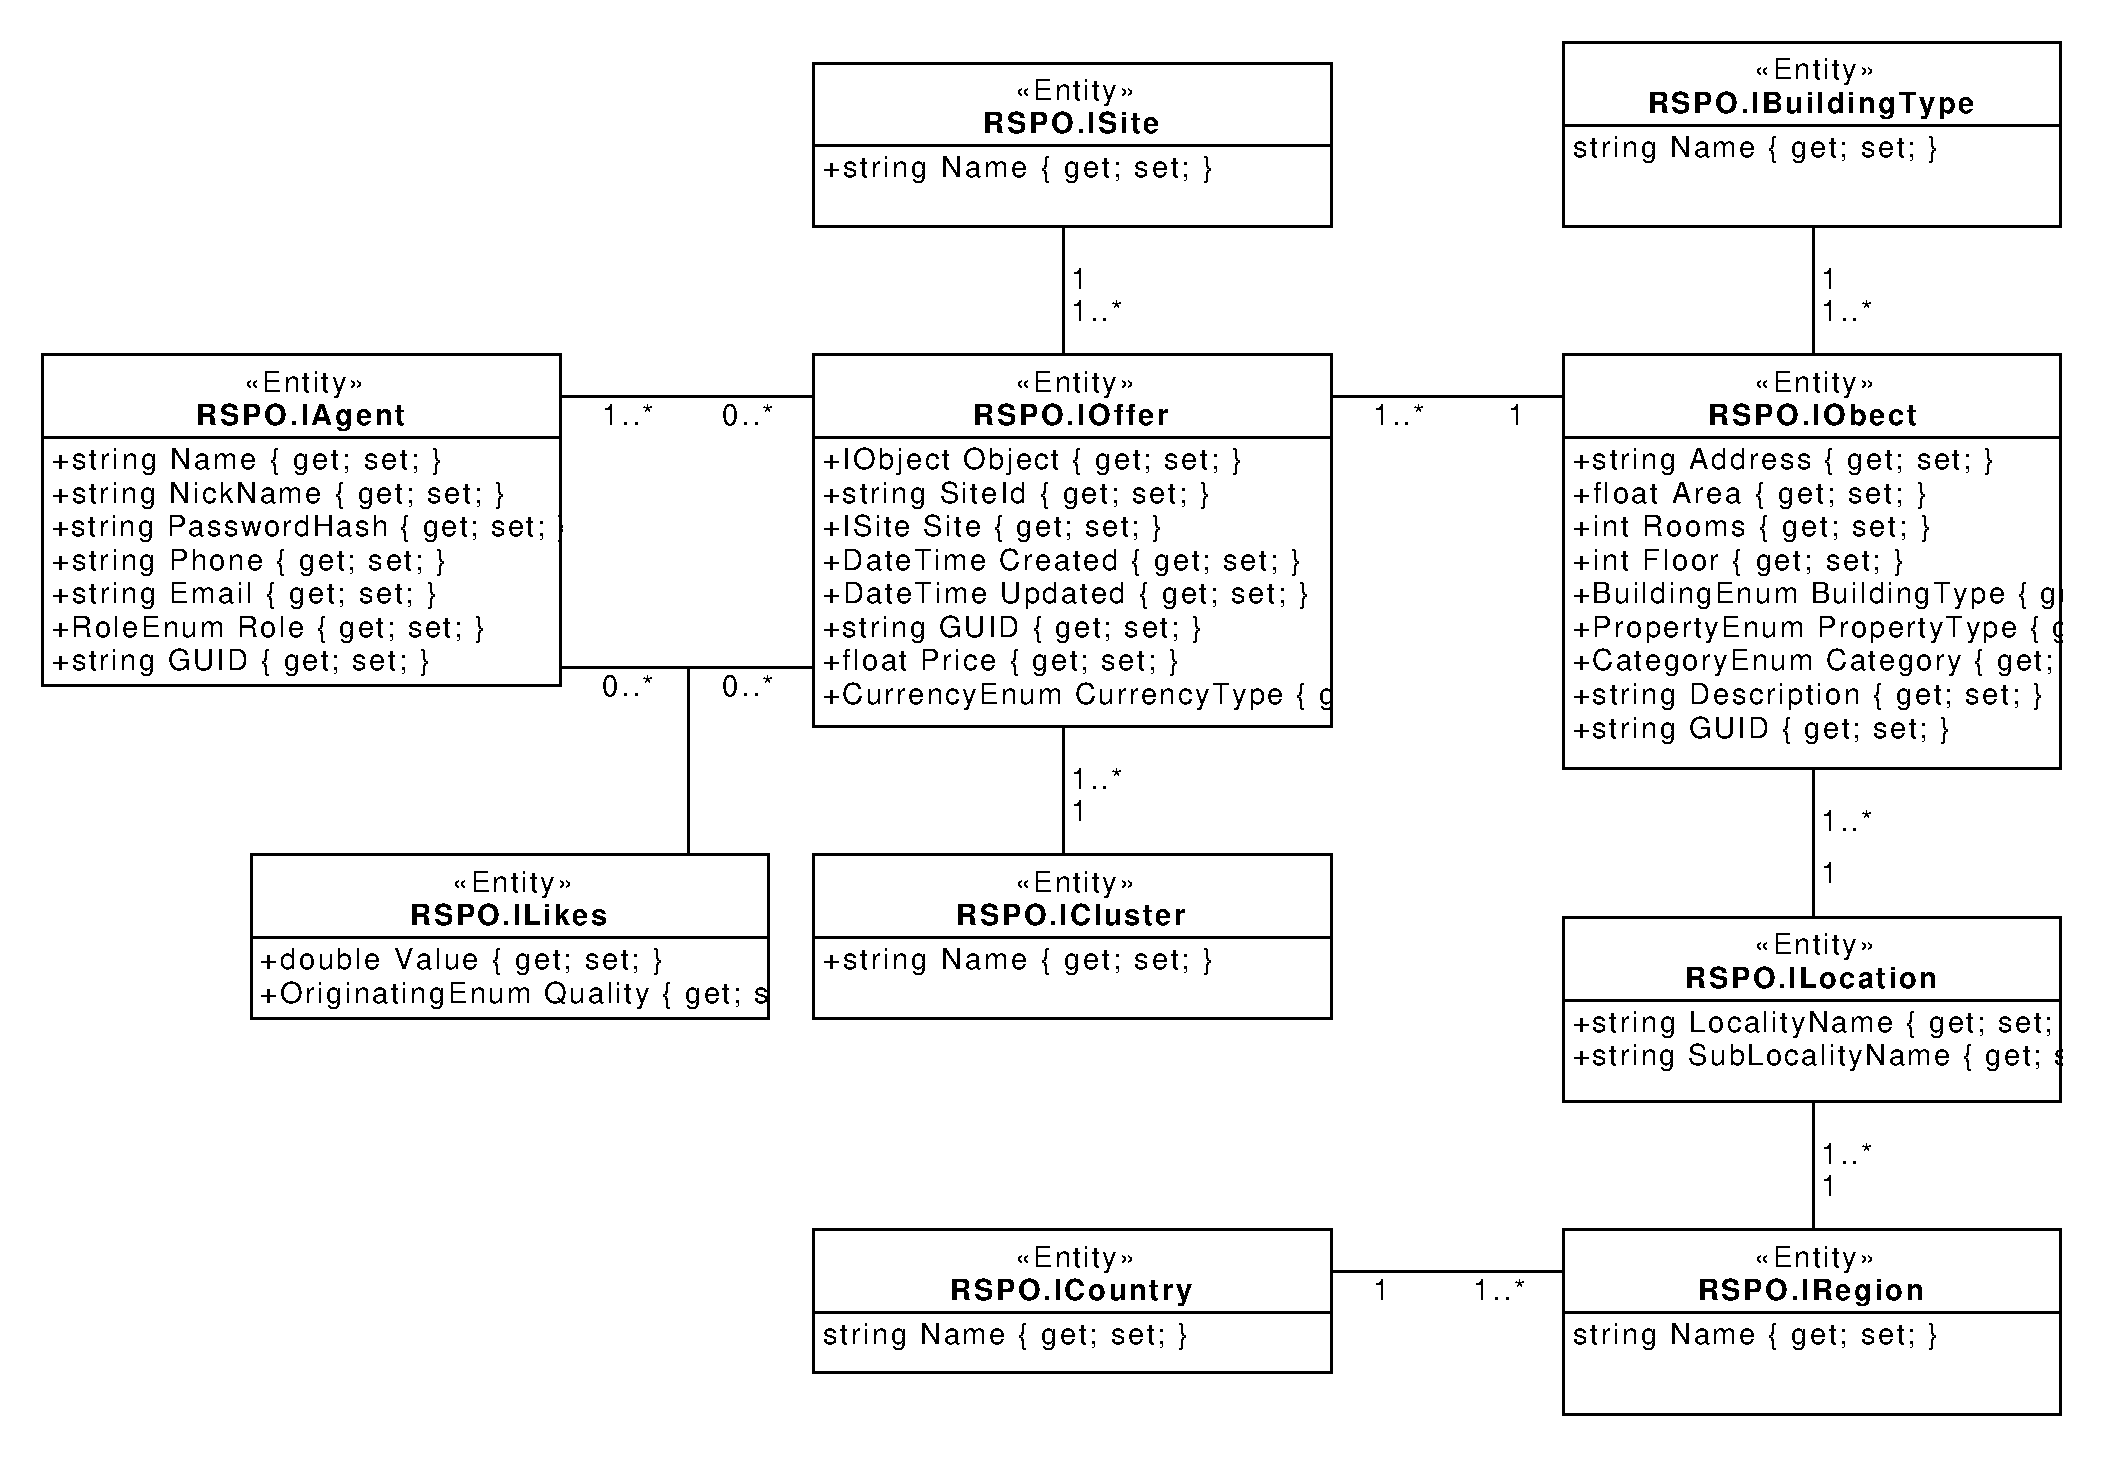
\includegraphics[width=1\linewidth]{class_diagram.pdf}

\end{frame}

\begin{frame}
  \frametitle{Discussion}
  The realty RS was tested by a number of buyers, none of them mentioned misbehavior of the system like spontaneous transitions from one class to another, or supplying empty sets of recommendations.

The presented experience shows that C\# .NET and MONO technologies and used techniques are well suitable for construction RS:
\begin{enumerate}
\item working in ``cold start'' conditions;
\item do not require user to register and authorize while implicit gathering information needed for recommendation generation;
\item testing systems are to be done in a local conditions to be able to check the results comparing with existing ``natural'' data;
\item using open-source technologies, modules and libraries.
\end{enumerate}

The obtained real estate RS implementation as well as the second project do not take advantage of the nowadays methods of R\&D development, which corresponds to current traditions.  Most attention is paid to preliminary data processing and obtaining minimal valuable product (MVP).
\end{frame}

\begin{frame}
  \frametitle{Conclusion}
  We presented results of two master degree projects.  The first one is finished, and the second one is on a half way.  Both systems have similar design, but rely on different RS techniques. Both systems use persistent object-oriented representation of application entities.

We have to solve ``cold start'' problem for both domains by creating taxonomies to consider classes as objects of users' interests.  Taxonomies of users are also created in Entrants' RS.

The described technique could be developed further by adaptation the standard directions such as:
\begin{itemize}
  \item development or adaptation of ontology of domain to extend search capabilities especially in students' courses domain;
  \item case based reasoning for the same domain;
  \item predictive modeling of attribute values for realty;
  \item providing geospacial data of infrastructural service organizations in the environment, \emph{e.g.} schools, kindergartens and shops.
\end{itemize}
\end{frame}

\begin{frame}{}
  \vfill
  \centering
  \Huge \textbf{Thank You for attention!}
  \vfill
\end{frame}


\end{document}













\begin{frame}{Batch processing}

  There is three basic models of industrial processes: \alert{continuous}, \alert{discrete}, and \alert{batch processing}.  The most complex one is the third, the batch processing.

  %\begin{examples}
    \includegraphics[width=0.9\linewidth]{pics/BatchProcessPFD.png}

  %\end{examples}

\noindent The figures are taken from \url{https://en.wikipedia.org/wiki/Scheduling_(production_processes)}

\end{frame}

\begin{frame}[fragile]{Batch processing}

  \begin{columns}
    \begin{column}{0.5\textwidth}
      \begin{block}{Batch description}
        \tiny
\begin{verbatim}
    Unit Procedure 1: Reaction
        Op 1: Charge A & B (0.5 hours)
        Op 2: Blend / Heat (1 hour)
        Op 3: Hold at 80C for 4 hours
        Op 4: Pump solution through cooler to
              blend tank (0.5 hours)
        Op 5: Clean (1 hour)
    Unit Procedure 2: Blending Precipitation
        Op 1: Receive solution from reactor
        Op 2: Add solvent, D (0.5 hours)
        Op 3: Blend for 2 hours
        Op 4: Pump to centrifuge for 2 hours
        Op 5: Clean up (1 hour)
    Unit Procedure 3: Centrifugation
        Op 1: Centrifuge solution for 2 hours
        Op 2: Clean
    Unit Procedure 4: Tote
        Op 1: Receive material from centrifuge
        Op 2: Load dryer (15 min)
    Unit Procedure 5: Dry
        Op 1: Load
        Op 2: Dry (1 hour)
\end{verbatim}
\end{block}
\end{column}
\begin{column}{0.5\linewidth}
    \includegraphics[width=1\linewidth]{pics/BatchCT2.png}
    \includegraphics[width=1\linewidth]{pics/BatchCT3.png}
    \includegraphics[width=1\linewidth]{pics/BatchCT4.png}
\end{column}
  \end{columns}
\noindent The figures are taken from \url{https://en.wikipedia.org/wiki/Scheduling_(production_processes)}
\end{frame}

\begin{frame}{Batch proceedings visualization}

\includegraphics[width=0.7\linewidth]{pics/BatchGantt1.png}

\hfill    \includegraphics[width=0.7\linewidth]{pics/BatchLabor1.png}

    \noindent The figures are taken from \url{https://en.wikipedia.org/wiki/Scheduling_(production_processes)}
\end{frame}


\begin{frame}{Modeling}
  Representing industrial system as discrete-event system (DES), as some other technical and natural objects, almost always we deal with consumption, production and concurrent temporal acquiring resources.

  Examples of the kind are
  \begin{enumerate}
  \item computer networks;
  \item resource allocation in computer cloud systems;
  \item automated manufacturing; air traffic control;
  \item robotic assembly lines;
  \item highly integrated command, control, communication, and information systems, \emph{e.g.}, groups of underwater unattended vehicles.
  \end{enumerate}

  \alert{Uncertainties} are classified in \alert{external} and \alert{internal}, \alert{event-based} and \alert{resource-based}.  Uncertainties, as events of DES generated by the environment of the industrial system, can be represented with game theory.  This representation will model the behaviors of external agents (\emph{e.g.} firms, teams, or individuals) under different \alert{competition} and \alert{collaboration} strategies.  Resource-based uncertainties represent usually crshortage of resources (utilities).
\end{frame}

\begin{frame}{Existing approaches}
  Aim of control is to retain IS near a \textbf{set point} or correspond to a \textbf{set of constraints}.
  \begin{itemize}
  \item Environment generates events, industry reacts. A set of reacting rules must be synthesized.
  \item Mean field games. Number of agents are infinite, continuous mathematic methods are applied.
  \item Predictive control, a model-based optimization. Model predicts the future states with \alert{receding horizon} strategy.
    \begin{itemize}
     \item \alert{Distributed cooperative control} of relatively
       independent subsystems. Lowering computational complexity.
     \item with limited resources and asynchronous coordination.
     \item with structural uncertainties (equipment failure, illness of staff). Resource reserves are accounted.
     \end{itemize}
  \item Fuzzy and neural network methods (blackbox).
  \end{itemize}

  We propose to represent IS with its environment as DES, which behavior described by resource-based games.  In this case we could apply methods of supervisor control synthesis in addition to the predictive techniques.

\end{frame}

\begin{frame}{Aim of the research}
\textbf{The aim is} the development of new methods of intelligent control synthesis for resource-driven DES with uncertainties is based on
\begin{enumerate}
\item new declarative means in aspects of: event occurrence, state change, resource consumption/production and acquiring, competitor behavior, \emph{etc}.;
\item devising approaches to visual definition of the model with UML, SysML, BPMN, CMMN;
\item development modular supervisors by means of logical inference;
\item adaptation of existing logical inference approaches to support resource-driven games;
\item devising a software for DES description and its computer simulation.
\item represent near-to-real manufacturing processes as RDDESU;
\item testing the methods and software in manufacturing control.
\end{enumerate}

\textbf{Using automation is due to the complexity and scale of the problem.}
\end{frame}

\begin{frame}[fragile]{Resource-based games}
\noindent  $S=\langle v_0,R,F \rangle,$ where $v_0$ is a multiset, $v_0=\{4\cdot(a,A),8 ⋅ (b, A), 9 ⋅ (c, A),$
  $6 ⋅ (a, B), 10 ⋅ (b, B), 3 ⋅ (c, B), 12 ⋅ (d, B), 1 ⋅ A\}$.

  \noindent  Rules, defining agents' behavior:\\
$(r_1^A): \{1 \cdot  A, 2 \cdot  (a, A), 1 \cdot  (b, A)\} → \{−1 \cdot  (a, B), −1 \cdot  (d, B), 1 \cdot  B\},$
$(r_2^A): \{1 \cdot  A, 1 \cdot  (a, A), 3 \cdot  (b, A)\} → \{−2 \cdot  (a, B), 1 \cdot  B\},$
$(r_3^A): \{1 \cdot  A, 1 \cdot  (a, A), 2 \cdot  (b, A), 3 \cdot  (c, A)\} → \{−1 \cdot  (b, B), −4 \cdot  (d, B), 1 \cdot  B\},$
$(r_1^B): \{1 \cdot  B, 3 \cdot  (a, B), 2 \cdot  (b, B)\} → \{−2 \cdot  (a, A), −1 \cdot  (b, A), 1 \cdot  A\},$
$(r_2^B): \{1 \cdot  B, 3 \cdot  (a, B), 2 \cdot  (b, B)\} → \{−4 \cdot  (c, A), 1 \cdot  A\}.$

\noindent Filter conditions:

\begin{columns}
    \begin{column}{0.45\linewidth}
$(C_1^A): (a, A) ≥ 2,$\\
$(C_2^A): (b, A) ≥ 4,$\\
$(C_3^A): (c, A) \to max,$\\
$(C_4^A): (d, B) \to min,$\\
$(C 5A ): (b, B) ≤ 2,$\\
\alert{$F_A = \{C_1^A,\ldots, C_5^A\}$ is A-\bfseries goal}.
    \end{column}
    \begin{column}{0.45\linewidth}
$(C_1^B): (a, B) ≥ 3,$\\
$(C_2^B): (b, B) ≥ 5,$\\
$(C_3^B): (c, A) \to min,$\\
$(C_4^B): (b, A) ≤ 3,$\\
\mbox{$$}\\
\alert{$F_A = \{C_1^B,\ldots, C_4^B\}$ is B-\bfseries goal.}
    \end{column}
  \end{columns}
\vfill
\noindent The example is taken from Igor Sherement's ICCS-DE~2020 paper \url{http://ceur-ws.org/Vol-2638/paper22.pdf}.
\end{frame}

\begin{frame}
  \frametitle{System modeling. SysML }
  \centering
    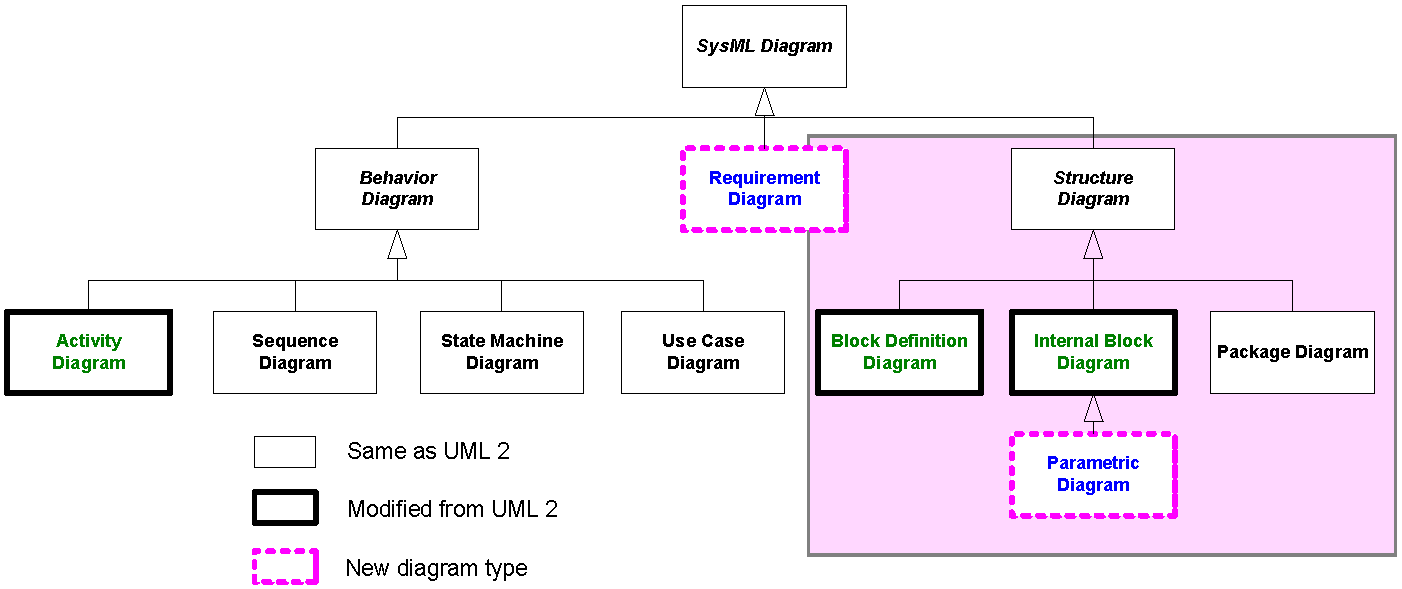
\includegraphics[width=1\linewidth]{qms-pics/diagrams.pdf}
\end{frame}
\begin{frame}
  \frametitle{System modeling. Requirements Diagram}
  \centering
    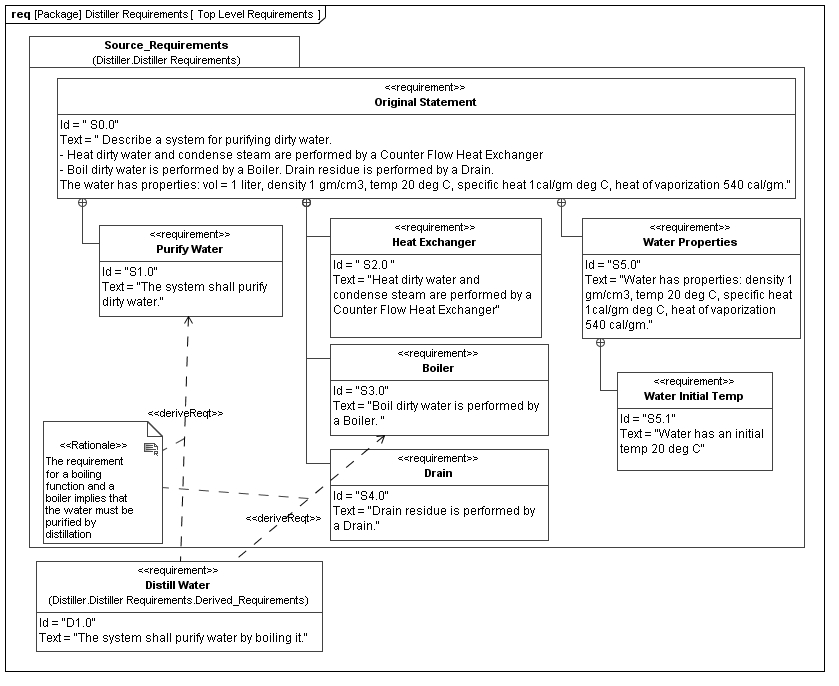
\includegraphics[width=0.9\linewidth]{qms-pics/req-ex.png}
\end{frame}
\begin{frame}
  \frametitle{System modeling. Parametric Diagram}
  \centering
    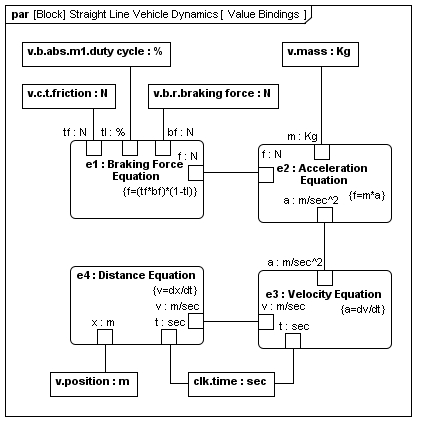
\includegraphics[width=0.7\linewidth]{qms-pics/par-ex.png}
\end{frame}
\begin{frame}
  \frametitle{System modeling. BPMN2.0}
  BPMN -- Business process modeling notation
  \centering
    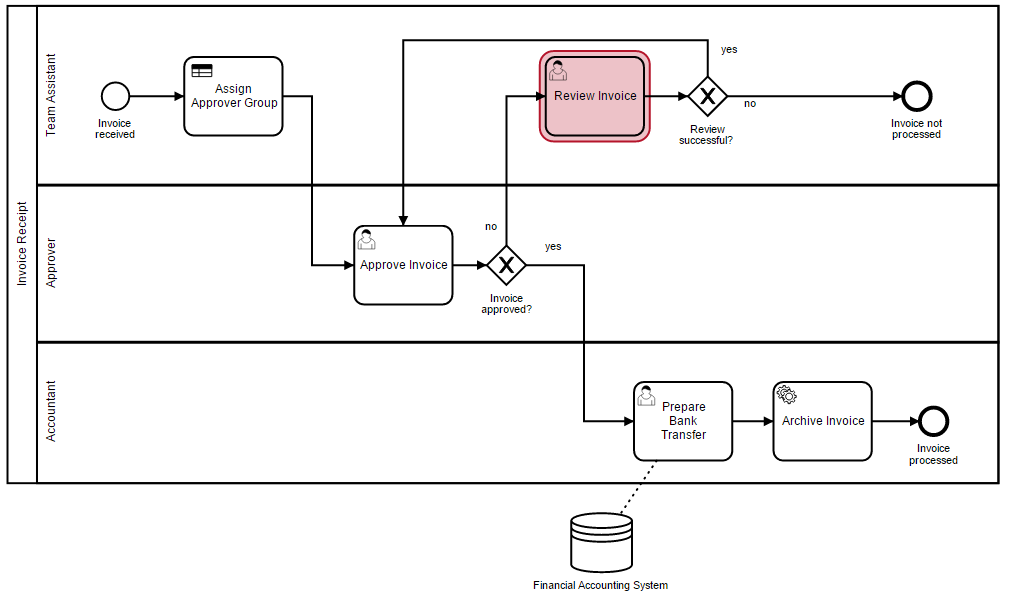
\includegraphics[width=1\linewidth]{qms-pics/bpmn.png}
\end{frame}
\begin{frame}
  \frametitle{System modeling. CMMN1.1}
  CMMN -- Case management model and notation
  \centering
    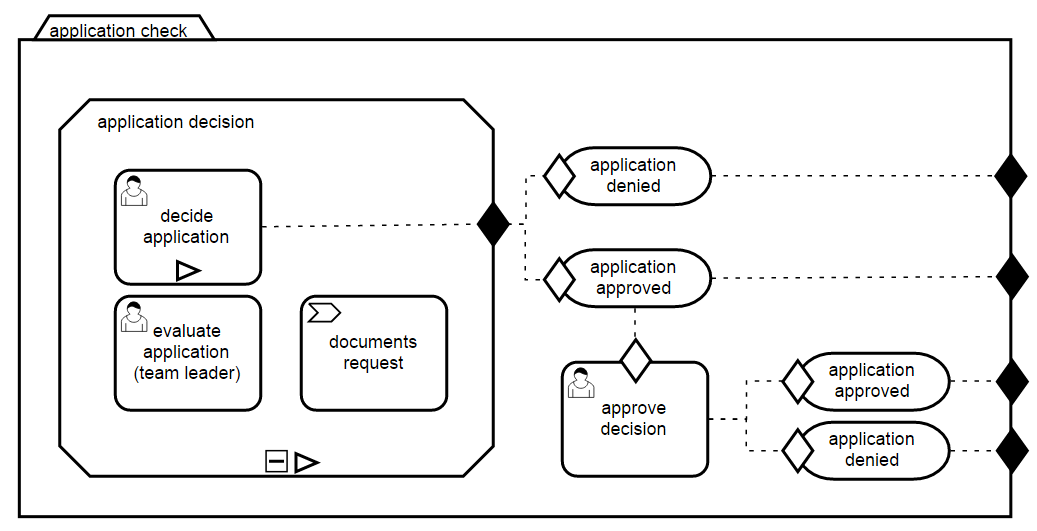
\includegraphics[width=1\linewidth]{qms-pics/cmmn.png}
\end{frame}


\begin{frame}{Control synthesis}
  \begin{enumerate}
  \item DES control is synthesized algorithmically by analysis the controlled automaton. The synthesized control (subautomaton) prevents occurring events shifting system out of admissible state set.
  \item Modifiers of inference rule the default strategy of PCFs were designed for that purpose. The control is synthesized while making proofs.
  \item If the synthesis is not possible, it shows structural elements, preventing the synthesis.
  \item The same was done for language representation of the DSS.
  \item Decentralized control tested on controlling formations of UAVs.
  \end{enumerate}
  Another way is use of forward-chaining inference like receding horizon in RTS mode, where inference stops as soon as time is up.  At each step set of constraint are tested, the admissible states form resulting trajectories and control.
\end{frame}

\begin{frame}{Further activities: Expected results}
\begin{enumerate}
\item A technique for representation complex of models, data structures.
\item Adaptation of standard visual notations (UML, SysML, \ldots).
\item Transformation of the visual models to the internal representation.
\item Methods of synthesizing supervisors for the DES on the base of automatic theorem proving in PCFs.
\item Device new techniques of constructive inferences constructions adopted to the subject of research.
\item Modular automated research software on the base of computer simulation of predictive control with our extensions.
%\item Techniques of the near-to-real manufacturing process formulation as complex of visual models will be developed.
%\item An extensive testing on real industrial processes.
\end{enumerate}
LNHU will perform the following activities:
\begin{enumerate}
\item Research of resource-driven multi-objective optimization: optimal set point and the coordinating multi-objective strategy.
\item Research of distributed predictive control for RDDESU systems with regards of industrial scale and complexity.
\item The establishment of visualization model of ethylene and polypropylene production.
\item Application of the proposed control techniques in petrochemical processes accounting the uncertainties.
\end{enumerate}

\noindent\textbf{The software aimed at CAE/CAM systems development for IS.}
\end{frame}

\begin{frame}{Conclusion}
  The talk was devoted to assess the applicability of existing methods, algorithms and software for construction of \textbf{automated research} software for synthesis of control for three-layer advanced industrial process control models.
  \begin{itemize}
  \item Planning, a composition of the bach processing line.
  \item Scheduling, execution of the plan, utilizing and producing resources.
  \item Control of dynamic of the scheduling with synthesis of DES control supervisors and admissible trajectories in the predictive control mode.
  \end{itemize}

  The enrichment of the convenient standardized two-level model with resource-based game theory enables us to decompose the sources of uncertainties ain a image and likeliness of industry modeling subunits as agents of multi-agent systems.

\end{frame}


%%% Local Variables:
%%% mode: latex
%%% TeX-master: "talk-2020-09-03-proposal.tex"
%%% End:
